\documentclass[DIV=calc, paper=a4, fontsize=11pt]{scrartcl} % Документ принадлежит классу article, а также будет печататься в 12 пунктов.
\usepackage{ucs}
\usepackage[T1,T2A]{fontenc}
\usepackage[utf8x]{inputenc} % Включаем поддержку UTF8
\usepackage[russian]{babel} % Пакет поддержки русского языка
\usepackage{titling} % Allows custom title configuration

%for frames
\usepackage{framed}

%For image using
\usepackage{graphicx}

%Numbering subsubsubsections etc
\setcounter{secnumdepth}{5}

%For code highlightning
\usepackage{listings}

%Further enumeration
\usepackage{enumitem}
\setenumerate[1]{label=\theparagraph.\arabic*.}
\setenumerate[2]{label*=\arabic*.}
\setenumerate[3]{label*=\arabic*.}


%For referencing within enumeration lists
\usepackage{enumitem}

%Packages for word-like comment style
\usepackage{todonotes}

%Package for images
\usepackage{float}
\floatstyle{boxed}
\restylefloat{figure}

%For a nicer reference
\usepackage{fancyref}

\usepackage{titlesec}


\titleformat*{\section}{\LARGE\bfseries}
\titleformat*{\subsection}{\Large\bfseries}
\titleformat*{\subsubsection}{\large\bfseries}
\titleformat*{\paragraph}{\large\bfseries}
\titleformat*{\subparagraph}{\large\bfseries}

%For some math formulas if needed
\usepackage{mathtools}

% Some nice visualization
%\usepackage[svgnames]{xcolor} % Enabling colors by their 'svgnames'
\usepackage{fullpage}
%\renewcommand{\headrulewidth}{0.0pt} % No header rule
%\renewcommand{\footrulewidth}{0.4pt} % Thin footer rule
% End visualization

%smart enumeration
\renewcommand{\labelenumi}{\arabic{enumi}.}
\renewcommand{\labelenumii}{\arabic{enumi}.\arabic{enumii}}


\title{Макет технического задания для салонов красоты (рабочее название - Beauty Booking или BB)}
\date{07/10/2014}

\begin{document}

\maketitle

\section{Описание проекта}
Сайт представляет собой платформу, на которой клиенты могут искать бьюти-услуги, а салоны и фрилансеры предлагать такие услуги. Сайт состоит из двух компонент - компонент для клиента представляет собой удобный поиск и бронирование похода к мастеру. Для мастера (салон или фрилансер) сайт представляет собой полноценный административный рабочий инструмент. Мастер может принимать заявки в режиме онлайн, вести учетную запись клиентов, получать заказы с сайта (с компонента для клиентов), продвигать свои услуги.
\subsection{Описание компонента для клиента}
Для клиента сервис собой представляет красивый сайт, позволяющий искать услуги по запросу клиента. Особенностью сайта является его полная адаптивность и облик мобильного приложения, который полностью копирует мобильную версию сайта (также и по функционалу). 
\\[0.5cm]
Подробнее о клиентской части позже, так как изначально разрабатывается часть для мастера.
\subsection{Описание компонента для мастера}
Мастер/салон может зарегистрировать себя на сайте, получив доступ к определенной части сайта, недоступной для обычного пользователя. Эта часть называется "кабинет". В кабинете мастер/салон может вести всю свою предпринимательскую деятельность, связанную с бьюти-услугами - принимать онлайн-заявки от клиентов, просматривать финансовые показатели, определять финансовые параметры услуг, проводить промо-акции, вести учетную запись клиентов, проводить рассылку для пользователей и многое другое (конкретный перечень в списке описания кабинета).
\subsection{Пользователи}
Пользователями системы являются люди, которые хотят получить бьюти-услуги (стрижку, маникюр, массаж...), а также люди, эти услуги предоставляющие (это могут быть отдельные мастера, а также салоны) - в дальнейшем будет использоваться обозначение "мастер", но под этим подразумевается как и фрилансер, так и компания.
\subsection{Конкуренты}
Текущие конкуренты сайта:
\\[0.5cm]
http://hairbook.ru - русскоязычная аудитория
\newline http://wahanda.com - аудитория Великобритании
\newline http://styleseat.com - американская аудитория

\subsection{Тарифы} \label{subsec:tariffs}
Сервис ГетБам подразумевает для салонов различные тарифы (список может пополняться)

\paragraph{Базовый тариф}
При базовом тарифе салон не платит абоненскую плату за сервис "тетрадка", при этом он платит комиссию за каждого клиента, который приходит с сервиса "зеркало" или через сервис "кнопка на сайте" (процент комиссии меняется в зависимости от выбранного тарифа - в базовом комиссия выше, чем в более высоких тарифных планах). Салону доступны стандартные модули (кокпит, календарь, список услуг, список клиентов, настройки). Также у данного тарифа самая высокая стоимость СМС.
На 30/03/2015 комиссия составляет 10\%. Стоимость СМС-сообщений составляет 1.5 рубля.

\paragraph{Тариф медиум}
Состоит из абонентской платы за тетрадку, но при этом комиссия за каждого клиента ниже. Выгодно салонам с высокой посещаемостью. Также цены на СМС-сообщения ниже.
На 30/03/2015 абонентская плата составляет 2400 рублей/месяц. Комиссия составляет 7\%. Стоимость СМС-сообщений составляет 1.2 руб.

\paragraph{Порядок оплаты}
Счета на СМС и абонентскую плату всегда выставляются в виде предоплаты.Если салон не оплачивает счет в течении 7 дней, не начисляем клиенту СМС и не переводим его (если это первый раз) на следующий тариф или возвращаем в базовый.
В случае неуплаты счета за комиссию в течении 7 дней, то перестаем выводить салон на Зеркале.

\section{Технические уточнения}

\subsection{Термины}

        \begin{itemize}
        \item Блок - некий визуальный элемент, выделяющийся либо графически (в виде рамок, очертаний), либо по смыслу (совокупность похожих элементов)
        \item Компонент - часть содержания, имеющего закрытое визуально представление. Одна страница сайта может состоять из нескольких компонентов.
        \item Фронтэнд - для пользователя видимая оболочка веб-страницы
        \item Бэкэнд - невидимые для пользователя математические алгоритмы
        \item CMS - все работы происходят на основе системы управления содержанием - CMS 1C Bitrix (1С Битрикс)
        \item Модуль - является описанием общего функционала, который не может быть классифицирован как привязанный к определенной странице. Он может встречаться на любой странице в любом месте. Модуль может состоять из нескольких компонентов. Также модуль может содержать в себе части логики фронтэнда и бэкэнда.
        \item Хэдер - верхняя часть сайта, обладающая определенной структурой, которая видна сквозняком на всех или почти всех страницах сайта. Также используется обозначение "шапка".
        \item Футер - нижняя часть сайта. Функционал аналогичен хэдеру. Также используется обозначение "подвал".
        \item Тетрадка - рабочее и финальное название для кабинета салона красоты.
        \item Зеркало - рабочее название для сайта, который доступен клиенту (позже этот сайт будет по-умолчанию доступен по адресу getbam.ru)
    \end{itemize}


\subsection{Технические требования к сайту}
Сайт должен быть адаптивным, поддерживать IE 8+ и использовать технологию композита.
Тут ещё больше технического бла-бла.


\section{Модули}
Каждую страницу, а также определенные составляющие страниц можно отключить или включить для разных групп пользователей по желанию администратора сайта. Так например модуль 'Финансы' включает в себя как и отдельную страницу со сводкой финансов, так и виджеты на других страницах, показывающие короткую статистику.
\subsection{Виджет для собственных сайтов} \label{subsection:widget}
Если у салона уже есть собственный сайт, то он может установить сниппет - js код - который позволит пользователям через данный виджет бронировать услуги. Данная бронь попадает, как и через главный сайт getbam в кабинет салона.
\\[0.5cm]
С технической точки зрения виджет должен отправлять post-request с параметрами салона (id) и параметрами клиента. 
Виджет состоит из выбора услуги, доступной в данном салоне, выбора времени и мастера (опционально).
В качестве настроек виджету можно задать базовые css-параметры, отвечающие за цвет (background) виджета, форму и цвет кнопки отправки. Также для более продвинутых пользователей нужно предоставить возможность редактировать css вручную.

\subsection{Проверка салона на честность}
Возможная проблема - салон записывает клиентов через систему, но как подходит очередь клиента, администратор салона (или фрилансер) нажимает на кнопку отказа (=клиент не появился). Для пресечения подобных мер необходимо реализовать модуль мониторинга, который будет агрегировать информацию по салонам и предоставлять её нам (как главным администраторам).

\subsubsection{Доверительный интервал}
Самая главная настройка 

\subsection{Чат}
Информация дополняется

\subsection{Сайт салона}
Конструктор сайта для салона. Позволяет задать базовые параметры по дизайну (цветовая гамма, вид кнопок), а также по наполнению (области для информации сайта - баннеры, услуги, акции и прочее). Данный функционал является наименее приоритетным.

\subsection{Финансы}

\subsection{Склад}
Модуль дорабатывается отдельно. Описание см. пункт \ref{subsec:warehouse}.

\section{Страницы}

\subsection{Сайт для клиента}

\subsubsection{Главная страница}

На главной странице, идя сверху вниз присутствуют несколько логических блоков. Первый - верхнее меню, позволяющее пользователю выбрать из категорий самых распространенных видов услуг. При нажатии на ссылку будет выпадать прямоугольный блок, который в свою очередь несет свой набор действий (утверждается). Также на уровне верхнего меню есть поиск и кнопки входа/регистрации для компании (регистрации для пользователя как такогого нет - пользователь может нажать на "войти" и там создать новую учетную запись).
\\Второй блок - область баннера, также содержит форму поиска процедуры. В самом низу данного блока ещё раз повторяется меню, аналогичное первому блоку. Пункты данного меню также открывают прямоугольные области.
\\Третий блок - рекомендации редакции. Некий слайдер топовых услуг. В первом релизе это полностью статичная информация.
\\Четвертый блок - меняем информацию под собственные нужды. Также статичная информация.
\\Пятый блок - топовые предложение от топовых студий (проплачивается студиями на основе хитрого алгоритма). В первом релизе статичная информация.
\\Шестой блок - футер: содержит подписку на ньюслеттер, ссылки на скачивание мобильных приложений, ссылки на соц.сети, ссылка на подстраницы.

\paragraph{Верхнее меню}

\subparagraph{Список категорий} \ref{subparagraph:categories}

При нажатии на один из пунктов верхнего меню появляется прямоугольная область, содержащая (утверждается - скорее всего ссылки на подкатегории, а также лучшие предложения из данной категории. Например если ссылка верхнего меню - "Волосы", то в прямоугольной области перечнем могут идти "Стрижка", "Наращивание волос", "Наворачивание бигудей". В качестве лучших предложений можно выводить салоны или рекламные продукты или ещё что-то, связанное с волосами). Прямоугольная область слегка прозрачная и открывается \textbf{под} верхнем меню. 

\subparagraph{Остальные ссылки}

Войти/Зарегистрировать бизнес - при нажатии на "войти" открывается также прямоугольная область, внутри которой расположена форма для входа. Также в этой области расположена кнопка "создать учетную запись", которая ведет на новую страницу, на которой пользователю доступны куча полей для непосредственно регистрации.
При нажатии на "зарегистрировать бизнес" перенаправляем пользователя на getbam.ru/business.

\paragraph{Область баннера}
\subparagraph{Поиск} Поиск является набором фильтров с возможностью поиска по значениям фильтра. Состоит из трех полей:

\begin{itemize}
	\item Услуга - выводим выпадающий список, поделенный на категории и подкатегории услуг. Но для подкатегорий выводим в списке не все, а только топовые (в первом релизе вручную указываем какие самые топовые). Для поиска доступны все подкатегории. (поле для поиска опционально)
	 \begin{figure}[H]
        \centering
        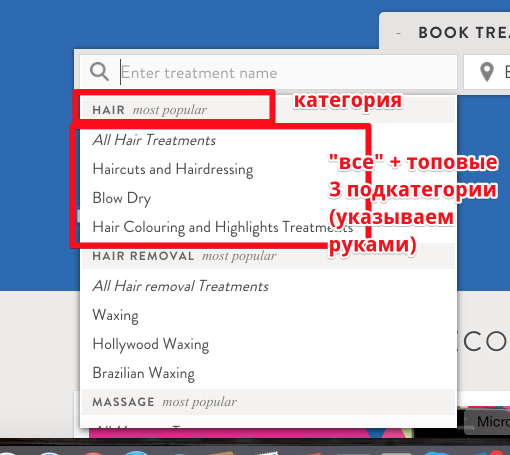
\includegraphics[width=320px]{search_field1.jpg}
        \caption{Пример списка на ваханде\label{fig:search_field1.jpg}}
        \end{figure}
        
     \item Местоположение - выводим список Московских станций метро и рядом "или рядом со мной" (запрашиваем геоположение пользователя) (обязательное поле)
     \item Дата - выбор даты. (опционально)
     \item Элемент-выбор цены (возможно слайдер) - позволяет выбрать цену на услугу (опционально)
     \item Кнопка "поиск" ведет на страницу с результатами поиска (СЕРП)
\end{itemize}

Поиск должен работать в том числе только с полем "местоположение", т.е. без даты и услуги. Таким образом я могу посмотреть что вообще доступно рядом со мной или в том месте, которое я как пользователь указал.

\subsubsection{СЕРП}

Показываем списком салоны, которые соответствуют запрошенным параметрам. Если по запросу доступно слишком большое кол-во услуг салона (например при запросе "все услуги по волосам" у салона 12 услуг), то всегда ограничиваем пятью услугами и оставшиеся скрываем.

	 \begin{figure}[H]
        \centering
        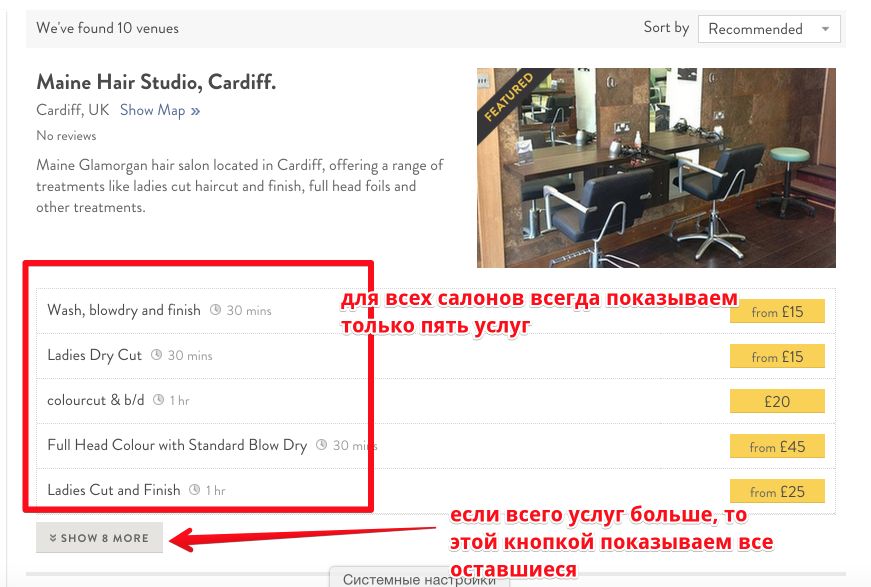
\includegraphics[width=320px]{serp1.png}
        \caption{Пример серпа на ваханде\label{fig:serp.png}}
        \end{figure}
        
При нажатии на цену открывается окно бронирования (см. пункт \ref{paragraph:app_booking}).
Дополнительные возможные действия на странце серпа - можно нажать на название салона и попасть на страницу салона.
\\[0.5cm]
На страницу серпа также можно попасть по ссылкам из меню категорий (получаем некий справочник - см. пункт \label{subparagraph:categories}). Смысл такой же - по запросу, например getbam.ru/places/hair (все салоны, которые предоставляют услугу из категории "волосы") или getbam.ru/places/hair/hair_cut (все салоны, которые стригут волосы).
\\[0.5cm]
Все салоны - getbam.ru/places
\\Страница конкретного салона - getbam.ru/places/salonName

\subsubsection{Страница салона}

\paragraph{Общий вид}

Общий вид делится на две колонки (соотношение grid - 8/2, по 1 слева и справа пустуют).
\subparagraph{Грид-колонка 8}
Сверху вниз - область баннера состоит из фотографий, которые загрузил салон у себя в ЛК -> Учетная запись.
\\[0.5cm]
За ним следует описание салона (которое также можно занести в ЛК -> Учетная запись у салона)
\\[0.5cm]
Далее следует перечень услуг салона с указанием названия, длительности и стоимости (указываем "от ХХ" если услугу делают несколько мастеров)

\paragraph{Окно бронирования}\label{paragraph:app_booking}
Самое важное окно для салона. Позволяет клиенту выбрать услугу и записаться на нее онлайн (а также оплатить).

\subparagraph{Общий вид} состоит из: области баннера с фотографиями услуги (если есть, указывается также салоном) или рыбной фотографией. Функционал можно взять один в один со страницы салона. Далее указываем стоимость в текстовом формате (опять же "от ХХ" если несколько мастеров/групп оказывают эту услугу) и время (также, "от ХХ минут" если мастеров/групп несколько).
\\[0.5cm]
Далее описание услуги и критерии возврата денег (см. пункт \ref{subsection:money_return})

\subparagraph{Колонка бронирования} показывает группы мастеров (если клиент выбрал в фильтрах на главной дату, то показываем только мастеров, которые работают в данную дату). Если в группе мастеров хотя бы один работает в выбранную дату, то группа доступна для выбора. Мастера без группы также доступны для выбора (на одном уровне с группой).

\begin{figure}[H]
        \centering
        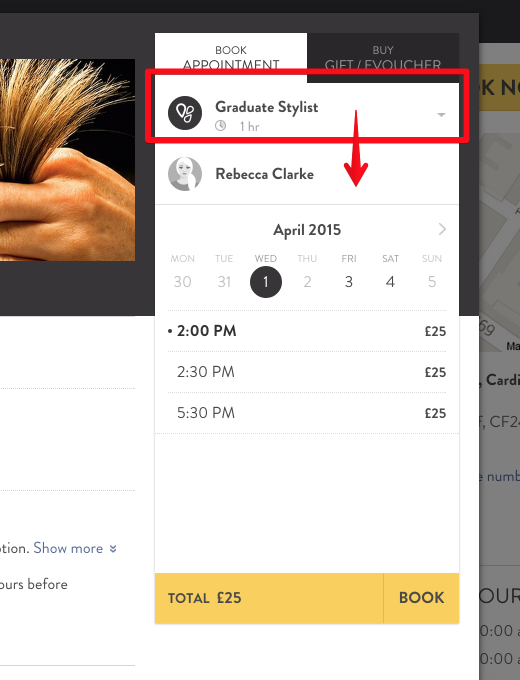
\includegraphics[width=320px]{before_booking.png}
        \caption{Пример выбора мастера на ваханде\label{fig:before_booking.png}}
        \end{figure}
        
После выбора мастера становится доступным выбор конкретного времени. Также клиент может просмотреть все доступные даты выбранного мастера, переключая по дням.
\\[0.5cm]
После выбора мастера и времени и нажатия на кнопку "бронировать" клиент перенаправляется на страницу оплаты.

\subsubsection{Страница оплаты}

\paragraph{Если клиент не зарегистрирован}
В данном случае страница содержит в себе 3 поля личной информации (имя, мэйл, телефон - все поля обязательны) и платежную информацию (в нашем случае ссылку на оплату Тинькова.

\begin{figure}[H]
        \centering
        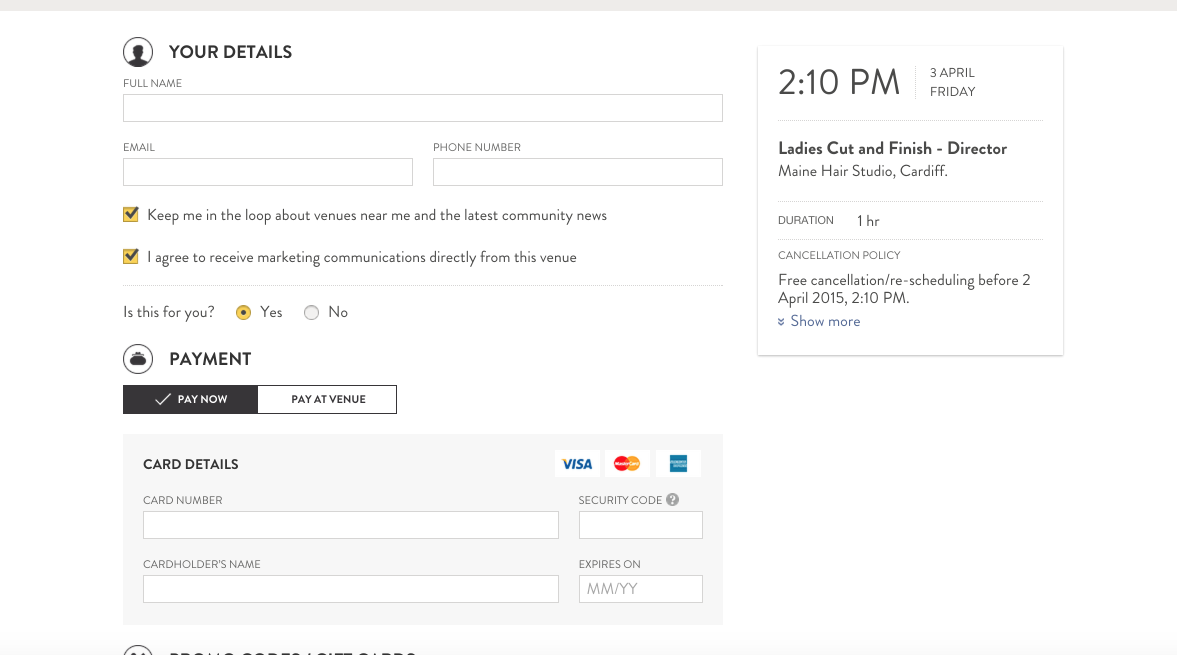
\includegraphics[width=320px]{payment_not_signed_in.png}        \caption{Оплата если пользователь не зарегистрирован\label{fig:payment_not_signed_in.png}
        \end{figure}
        
Также данная страница содержит в себе небольшую сводку по всему заказу.

\paragraph{Если клиент зарегистрирован}
В данном случае странице выглядит идентично как и в случае выше, но поля клиента (имя, мэйл, телефон) автоматически заполнены.

\paragraph{Страница подтверждения оплаты}
После оплаты перенаправляем сюда клиента, показываем - успешная была оплата или нет.

\subsubsection{Личный кабинет клиента}
\paragraph{Страница регистрации}
\paragraph{Страница напоминания пароля}
\paragraph{Главная страница}
\subparagraph{История посещений}
\paragraph{Редактирование данных}

\subsubsection{Идеи}

\paragraph{Ответственное бронирование}
Вступительный текст для пользователя - "Просьба бронировать ответственно. Часто салоны представляют собой независимых мастеров, для которых каждый отказ является сильным ударом. Мы знаем, что планы меняются, и если вы не в состоянии прийти на встречу, пожалуйста, поступите правильно и предупредите их как можно раньше. Если вы выбрали опцию "оплатить при встрече" и не появились в салоне, то в следующий раз эта опция будет заблокирована для вас. Надеемся на ваше понимание.

\paragraph{Проверка на доступность мастера}
При отправки подтверждения на услугу (т.е. на странице выбора мастера, даты и времени) программа должна проверять доступность мастера в указанное клиентом время. При этом сама проверка проходит непосредственно как только клиент выбрал все три параметра. Если возникает ошибка, то клиенту показывается сообщение об ошибке "К сожалению кто-то быстрее вас забронировал эту услугу. Пожалуйста, выберите другое время или другого мастера". Клиент нажимает на "ок" и возвращается к форме выбора времени и мастера, все другие данные при этом должны сохраняться.
\\[0.5cm]
Это задумано для того, что бы избежать двойных занесений если 1) другой пользователь быстрее забронировал эту услугу у того же мастера в то же время, что и первый пользователь или 2) салон сам занес нового клиента к тому же мастеру в то же время.
\\[0.5cm]
Также необходимо показывать таймер времени, который будет отсчитывать 15 минут на бронь, что бы клиент мог оплатить в это время (т.е. в течении 15и минут никто не может посягнуть на выбранное время)


\subsection{Кабинет студии}

\subsubsection{Кокпит студии}
Данный раздел кабинета мастера представляет собой сводку важных действий и информации для работы мастера. Делится на несколько частей - быстра сводка с фильтрами по дате, очередь клиентов, быстрая статистика по услугам и мастерам, быстрая статистика по финансам и клиентам.

\paragraph{Быстрая сводка} 
состоит из - под кнопки оформленных - блоков, показывающих следующую информацию:

    \begin{enumerate}          
        \item Клиенты на подходе - кол-во клиентов, которые придут в ближайшее время. Стандартно идут ближайшие 4 клиента с возможностью подгрузки ещё 4 и так итеративно до подгрузки всех клиентов текущего дня.
        \item Загрузка - рассчитывается из графика мастеров на основе выбранного фильтра по времени. Если фильтр - 'сегодня', то расчет происходит следующим образом: рабочие-часы-мастера/кол-во-заказанных-услуг*(время-услуги+пауза-между-услугой). Формально выглядит так: 
            $$
            L_m = \frac{W_m}{\sum n_m * (l_n + P_n)}
            $$
Где $L_m$ = загрузка конкретного мастера(в процентах), $W_m$ = рабочие часы мастера $m$ (управляется в настройках), $n_m$ = услуга $n$, забронированная на мастера $m$, $l_n$ = длинна услуги $n$ в минутах (управляется в настройках услуг), $P_n$ = время перерыва для услуги (управляется в настройках, может быть равно нулю). $n$ идет от 1 до $N$, где $N =$ последняя услуга дня мастера $m$. $m$ идет от 1 до $M$, где $M$ = общее кол-во занятых мастеров.
\\[0.5cm]
При выборе других фильтров расчет происходит идентично, только $n$ охватывает не только услуги одного дня, а все услуги выбранного фильтра.
        \item Ожидаемая прибыль за выбранный период времени является ожидаемой суммой по всем (предварительным) заказам на выбранный период. Заказ всегда является предварительным до тех пор, пока мастер не подтвердит фактический приход клиента. Формальная формула для одного мастера:
            
            $$
            I_m = n_m * c_n
            $$
Где $I_m$ = возможный приход мастера за выбранный период, $c_n$ = стоимость услуги $n$. Общий доход является суммой всех доходов по каждому мастеру:

            $$
            I = \sum_{m=1}^M I_m
            $$

        \item \label{paragraph:add_new_client}Добавить нового клиента/запись - вызывает всплывающее окно, позволяющее быстро создать нового клиента (с записью если необходимо). Такая функция необходима, если клиент не использует онлайн форму, а напрямую звонит или приходит в салон. При этом всплывающее окно позволяет внести ФИО и телефон (и если находит уже существующего человека по какому-либо из этих параметров, то позволяет выбрать его и прикрепить запись на услугу к конкретному лицу, если не находит, то создает новую запись). Также можно ввести мастера, если клиент сразу знает, к кому хочет попасть (при этом всплывает ещё одно окно, показывающее распорядок дня этого мастера), если нет, то на этом регистрация аппойнтмента заканчивается.

    \end{enumerate}

\paragraph{Очередь клиентов} \label{paragraph:plashki}
После быстрой сводки следует блок с очередью клиентов. В данном блоке плашками отображаются ближайшие клиенты на подходе. Плашки сортируются по дате актуальности, т.е. самые актуальные клиенты, которые вот-вот должны подойти отображаются сверху. Если клиент выбрал при онлайн-заявке уже конкретного мастера, то фотография мастера также отображается в плашке справа. Если клиент мастера не выбрал, то сотрудник может сам назначить мастера для клиента. Для этого он должен нажать на плашку и в правой области блока отобразятся фотографии мастеров, которые доступны для выбранной клиентом услуги в выбранное клиентом время. Сотрудник затем перетягивает фотографию мастера на плашку клиента, тем самым закрепляя мастера за клиентом. Для фрилансеров по-умолчанию работает автоприкрепление, так как они являются единственными мастерами.
\\[0.5cm]
В данную очередь попадают клиенты, как занесенные мануально администратором (См. пункт \ref{paragraph:add_new_client}), как и пришедшие с сайта getbam или через виджет на собственном сайте салона (См. пункт \ref{subsection:widget})
\\[0.5cm]
В плашке можно подтвердить приход клиента или сообщить о его отказе (при подтверждении и отказе перерасчитывается финансовые параметры, так как оценочная сумма обновляется уже подтвержденными данными). Автоматически отказы не происходят. Так, мастера, которые забыли подтвердить приходы клиентов, или если у них не хватило времени, могут сделать это в любое удобное время.
\\[0.5cm]
В плашке отображается дополнительно следующая информация по клиенту:

    \begin{enumerate}
        \item Иконка с полом (М/Ж)
        \item Категория услуги и услуга (например: волосы - окрашивание)
        \item Имя клиента
        \item Время забронированной услуги
    \end{enumerate}
    
\paragraph{Быстрая статистика по услугам и клиентам}
Данная область позволяет получить быстрый доступ к самым востребованным данным - статистике по услугам и статистике по мастерам. Область поделена на два блока (услуги и мастера). В будущем область будет настриваемой, что бы пользователи системы могли выводить в области некие виджеты.

\subparagraph{Услуги}
Для услуг необходимо отображать топ X (X управляется в настройках, по умолчанию равно 10) услуг, которыми пользуются клиенты. При этом необходимо считать как и брони (т.е. даже если бронь отменяется, в счетчик услуги идет +1) так и мануально созданные услуги.

\subparagraph{Мастера}
Аналогично предыдущей области, если клиент выбрал мастера при онлайн-заявке или назвал мастера сразу при звонке, считается рейтинг мастеров.

\paragraph{Быстрая статистика по финансам и посетителям}
Данная область расположена под блоком очередь клиентов. Область в будущем также будет настриваемой, что бы пользователи системы могли подключить свои собственные виджеты.
\subparagraph{Финансы}
Статистика по финансам показывает сколько денег было заработано через онлайн-заявки (т.е. сколько денег было заработано по полному пройденному циклу заявки - от получения до подтверждения прихода клиента).
\subparagraph{Посетители}
Статистика посетителей показывает сколько клиентов просмотрело на сайте ББ любые доступные услуги данного мастера.

\subsubsection{Календарь}
Календарь позволяет просматривать загруженность всех мастеров на день или неделю. Дополнительной фильтрации календарь не предусматривает (даже при двух мастерах вид на месяц будет заграможден), но при этом пользователь может переходить между неделями/днями. Также пользователь может скроллить между мастерами, если их столбцы не помещаются на одном экране.

\paragraph{Поиск мастера и услуги} \label{paragraph:calendar_filter}
Для больших студий актуально - поиск мастера и услуги. По сути это является фильтром для вида календаря. По умолчанию видны все мастера и все услуги.
\paragraph{Добавить новую запись}
При нажатии на дату в календаре появляется всплывающее окно добавления записи. При этом должны также учитываться результаты фильтров из пункта \ref{paragraph:calendar_filter}, т.е. если выбран мастер, то в попапе в выпадающем списке данный мастер также уже выбран. Всплывающее окно делится на две закладки - услуга&мастер и клиент. При этом на закладке услуга&мастер доступно поле поиска уже сущесвующих клиентов, и если таких нет, то программа показывает подсказку "такой клиент не найден, создать нового?". Если пользователь нажимает на данную подсказку, то он переходит во вторую закладку и может там создать нового клиента (при этом данные из запроса должны перениматься). Т.е. если я в первой закладке ищу "Маргарита Туева" и такой клиент не находится, то после перехода на вторую закладку ФИО должны быть уже заполнены значением "Маргарита Туева". 
\paragraph{Выбор даты}
Небольшой виджет календаря в левом сайдбаре позволяет выбрать конкретную дату, на которую при выборе пролистывается основной календарь. Также виджет поддерживает ссылки на недели (т.е. можно нажать на неделю и календарь пролистает до этой недели).
\paragraph{Вид календаря}
Календарь представлен по умолчанию видом на день, где в первом столбце идут дни/текущий день, а в последующих столбцах идут часы (по умолчанию один отсек равен часу, т.е. 8-9, 9-10, 10-11 и т.д.). Смысл системы схож с временной линией (timeline).
\\[0.5cm]
При виде недели и если аппоинтменов больше (больше плашек), чем высота дня, то появляется дополнительный элемент, при нажатии на который выбранный день раскрывается (скроллинг вниз) до тех пор, пока не будут видны все плашки дня.
 

\subsubsection{Услуги}

На странице располагаются списком все услуги, которые оказывает салон. Все услуги сервиса ГетБам деляться на 9 категорий:

\begin{itemize}
	\item Волосы
	\item Лицо
	\item Тело
	\item Ногти
	\item Загар
	\item Эпиляция
	\item Массаж
	\item СПА
	\item Другое
\end{itemize}

По умолчанию администратор салона видит пустой список с возможностью занести услугу, нажав на кнопку "добавить услугу". При этом открывается всплывающее окно, позволяющее занести все необходимые данные услуги. Данный попап идентичен с попапом редактирования услуги.

\paragraph{Редактирование/Добавление услуги} \label{paragraph:edit_service}
При нажатии на создание новой услуги или при нажатии на уже существующую услугу открывается всплывающее окно со следующими полями:

\begin{itemize}
	\item Общая категория (из вышеперечисленных 9) (не редактируется салоном)
	\item Подкатегория услуги (не редактируется салоном)
	\item Индивидуальное название (по умолчанию дублирует название подкатегории), которое салон может задавать сам
	\item Стоимость услуги с возможностью назначения различных групп мастеров и различных цен этим группам
	\item Перечень мастеров, кто принимает онлайн-заявки на данную услугу
	\item Список опций - когда доступна данная услуга на Зеркале, в какие дни на услугу можно записаться, тип продажи (ваучер, оплата...)
	\item Доп. описание - "что следует знать" (просто интересная информация) и "ограничения" (описание алергий всяких)
	\item Какой "предзаказ" у данной услуги (время + причина)
\end{itemize}

\paragraph{Предзаказ услуги}

Для специальных услуг должна быть опция, позволяющая указать время, которое минимум должно пройти прежде чем клиент сможет фактически прийти на эту услугу. 
\\[0.5cm]
Пример - для определенной услуги нужно заказать особенно дорогую косметику, которую привозят только через день после заказа. Соответственно сегодня в 10:00 я не смогу забронировать данную услугу на 12:00, а только на самое ранее 10:00 следующего дня.

\paragraph{Быстрое добавление услуги (визард)} \label{paragraph:appointment_wizard}
Визард представляет собой несколько чередующихся всплывающих окон, которые позволяют занести все необходимые услуги сразу. Для этого в первом окне пользователь может выбрать категории услуг и отметить нужные ему подкатегории чекбоксами.
\\[0.5cm]
Список подкатегорий можно сортировать по алфавиту и по популярности. Популярность считается по большинству занесений всех услуг всех салонов.
\\[0.5cm]
Далее для каждой услуги пользователь может назначить цену, длительность и мастеров, которые выполняют эту услугу. При этом цена задается стандартная (для всех мастеров), длительность задается также стандартная (для всех мастеров).

		\begin{figure}[H]
        \centering
        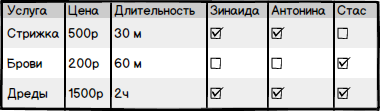
\includegraphics[width=320px]{add_appointment_wizard_p1.png}
        \caption{Примерный вид быстрой обработки всех отмеченных ранее услуг\label{fig:add_appointment_wizard_p1.png}}
        \end{figure}


\subsubsection{Финансы}\label{subsubsec:finance}
На странице расположены три типа фильтра и область для показа (визуального) результата (типов всего три - столбцы, пирог и диаграмма). Фильтры трех типов:
По направлению - затраты против доходов, оборот, прибыль
По параметрам компании/клиентов - [пусто], услуги, пол клиента, сотрудник, марка косметики
По дате - неделя, месяц, квартал, год
\\[0.5cm]
Все три типа можно совмещать, т.е. получить например график оборота по марке косметики за квартал или затраты vs. доходы по полу клиента. 
\\[0.5cm]
По разным направлениям показываем разные типы визуальных результатов. Например для затраты против доходов для нескольких сотрудников пироговый чарт не имеет смысла. Правило, как показывать когда какие чарты - всегда видна диаграмма+столбцы. Если направление выбрано 'затраты против расходов' и в параметрах более одного наименования, то не показываем pie-chart. Во всех остальных случаях показываем также pie-chart. (При выборе параметра 'пусто' график строится без фильтрации по услугам, клиентам и прочего.

\paragraph{Выписка по процентам, заработанным мастерами}
По итогам месяца (недели/квартала) или с промежутка последней выгрузки администратор салона может сгенерировать отчет, сколько каждый мастер заработал сверх оклада процентов за проделанные услуги.

\paragraph{Процент мастеру с услуги}
Тут возможны 2 варианта:
\begin{enumerate}
	\item Сначала в разделе 'услуги' тетрадки, при добавлении услуги, нужно дать возможность выбрать какой процент от стоимости услуги перепадает мастерам (всем, кто будет привязан к конкретной услуге).
	\end{enumerate}
	
	 В разделе "настройки - мастера" тетрадки, при добавлении мастера:
	\begin{enumerate}
	\item нужно дать возможность прикрепить мастера к конкретной услуге 
	\item дать возможность настроить индивидуальный процент со всех услуг, куда он будет прикреплен (может быть он неким рангом выше и имеет процент с услуги выше чем остальные или наоборот ниже)
\end{enumerate}


\subsubsection{Клиенты}
На данной странице отображены клиенты. Помимо табличного представления самих клиентов на странице возможен поиск клиентов, набор определенных быстрых действий (касающихся всех клиентов). 

\paragraph{Быстрые действия с клиентами} Также на странице можно совершить действия, такие как: создать рассылку, что-то ещё \todo[inline]{Что можно ещё добавить? Скидки определенным клиентам?}

\paragraph{Поиск} По клиентам должен работать поиск, поиска принимает фио, мэйл, дату визита и телефон. Он должен работать в режиме подсказки и без строго заданной маски. Т.е. телефон +7 903 227-88 74 должен найтись и по 8874, и по 8903227 и по 8 903 227 88 74 и по 8(903)227-88. 

\paragraph{Обзор клиентов} Клиенты выводятся на данной странице в табличной форме. Из столбцов доступны - ФИО, мэйл, телефон, последнее посещение, оборот с клиента (оборот настраивается, видно ли всем или нет. По умолчанию видно администратору), кол-во букингов

\paragraph{Ипорт клиентов} \label{paragraph:import_clients}
(На будущее) - необходимо опция импорта клиентов по формату CSV, XLS, XLSX, а также поддержка следующих систем (если нужно - добавить список этих систем). Для импорта нужен небольшой визард, который подскажет клиенту, как должен выглядеть файл, какие колонки должны быть где.

\paragraph{Опции каждого клиента} Нажав на конкретного клиента администратор сайта может открыть его карточку - на карточке доступны такие действия, как просмотреть и одновременно редактировать клиента, назначить аппойнтмент или удалить его. При просмотре данные подгружаются сразу в формате редактирования и доступны поля, такие как - аллергия, любимые направления, примечания (примечания видны при назначении нового апойнтмента), имя, телефон, эл.почта, подтверждение о согласии на получение рассылки, пол, день рождения. Также для клиента можно назначить из его карточки новый аппойнтмент.

\subsubsection{Склад} \label{subsec:warehouse}
Пока разрабатывается

\subsubsection{Помощь}
Данный раздел делиться на два подраздела - FAQ (часто задаваемые вопросы) и службу техподдержки через тикеты). 

\paragraph{FAQ}
Стандартный вид - частозадаваемые вопросы, которые находятся в свернутом режиме. Нажав на вопрос, ответ 

На данной странице администратор сайта может просмотреть номер службы техподдержки, а также направить писменный запрос. Для всех запросов заводятся тикеты, статус которых пользователь может просматривать. Тикеты делятся на актуальные, закрытые и отклоненные.

\subsubsection{Отчеты}
Отчеты представляют собой расширенный список данных по финансовым параметрам. Они представляют собой таблицы, по которым строятся графики из пункта (\ref{subsubsec:finance}). Таблицы можно получить по следующим данным: услуга, клиент, пол клиента, мастер, дата, время(длительность), прибыль. 
\\[0.5cm]
Для пользователя по умолчанию доступны следующие быстрые фильтры для отчетов: 
    \begin{itemize}
        \item Расходы vs. доходы/Прибыль/Оборот за месяц за месяц/квартал/полугодие/год
        \item 
        \item 
    \end{itemize}


\subsubsection{Настройки салона}

\paragraph{Добавление/редактирование мастеров}
В настройках можно добавлять/удалять мастеров, назначать каждому мастеру заранее указанные услуги и изменять общие данные мастера. Мастеров можно группировать (например начинающие мастера, продвинутые или профи)

\subparagraph{Профиль мастера} \label{subparagraph:masters_profile}
Доработка на будущее - в профиле мастера выводить все услуги, которые осуществляет мастер. Здесь же сделать возможным добавить услугу для конкретного мастера (с настройками услуги, такие как длительность и цена) и сделать возможным отмечать, какие из этих услуг доступны для бронирования онлайн.

\paragraph{Рабочее время}

Рабочее время - устанавливается рабочее время салона, индивидуально для мастеров а также допустимые паузы между приемами мастера. Для мастеров доступны два типа настроек времени - фиксированные (выбор дней) и гибкий (выбор графика, например 2 через 2).
\\[0.5cm]
Также каждому мастеру можно установить "блоки неработы", т.е. временные промежутки, которые могут быть произволными, во время которых мастер не работает (так, например, можно установить обеденный перерыв или короткую пятницу или ещё что-то)

\paragraph{Оплата}
Сервисы оплаты позволяют добавить различные способы оплаты, которые становятся доступными клиенту - опций на данный момент только две "Оффлайн" и "Онлайн". 

\subsubsection{Общие настройки (личный кабинет)}
Страница имеет несколько закладок (табов), по умолчанию открывается первый - лицевой счет.

\paragraph{Учетная запись}
На данной странице необходимы:

\begin{itemize}
	\item Загрузка и смена логотипа салона + также его превью
	\item Загрузка, смена и превью фотографий самого салона
	\item Редактирование названия салона (салон указывает при создании)
	\item Тип бизнеса (просто выводим, менять нельзя, только после обращения в службу технической поддержки)
	\item Фактический адрес салона (также просто выводим, редактирование только через обращение в ТП)
\end{itemize}

\paragraph{Счета}

На данной закладке видны текущие счета салона с возможностью оплатить онлайн кнопкой "перейти на оплату" (пользователь переходит на страницу агрегатора платежей, например PayOnline). Нажатие "загрузить ещё" подгружает все оплаченные счета. Также "плашки" со счетами имеют разный заставочный фон. Оплаченные счета - зеленый. Счета на подходе - оранжевый, просроченные счета - красный. Для юрлиц возможно также составление счета на оплату. При этом пользователю локально на компьютер скачивается стандартная версия текущего счета - происходит это при нажатии на "скачать счет" внутри "плашки".

Если агрегатор отдает данные об оплате, то сохраняем их также (выбранный метод оплаты и согласен клиент на периодическое списание денег)

\paragraph{Тарифы}

\paragraph{Лицевой счет}
На данной закладке пользователь видит номер лицевого счета, а также информацию о выбранном и всех доступных тарифах. Более детальную информацию о тарифах смотреть в соответствущем разделе (пункт \ref{subsec:tariffs}).
\\[0.5cm]
Клиент видит информацию о своем тарифе в красивом визуальном представлении (подствечивается его тариф) с перечнем того, что входит в тариф (также см. детальную информацию о тарифах - пункт \ref{subsec:tariffs}), также для среднего тарифа существует отметка "Самый популярный тариф" со сноской от какого кол-ва поситителей в месяц этот тариф становится выгоднее базового.

\paragraph{Финансы(денежные потоки)}
В закладке финансы администратор может просматривать детальную выписку по всем транзакциям, по аналогии с детализацией счетов мобильных операторов. По умолчанию идет перечень по месяцам, на каждый месяц можно нажать и раскрыть более детальную информацию за месяц. Доступны следующие столбцы информации:
\\[0.5cm] Клиент, мастер, когда была осуществлена услуга, тип услуги, ее цена и наша комиссия
\\[0.5cm] Также в финансах видна информация о купленных смс-уведомлениях (общий вид - сколько потрачено всего, сколько было куплено, сколько осталось, а также, аналогично с финансовой информацией - таблица, показывающая когда, на какой номер, с каким текстом ушла какая смс)
\\[0.5cm] Каждый из списков (по услугам и по смс) можно экспортировать в CSV.

\paragraph{Документы}
Перечень документов, делится на акты и счета-фактуры. Можно скачивать.

\paragraph{Рейтинг и комментарии}
На данной закладке администратор может просматривать общую информацию по рейтингу салона, так и отдельные комментарии. 
\\[0.5cm]Общая информация по рейтингу содержит в себе общий рейтинг салона, место по рейтингу в округе в радиусе 2 км, место по рейтингу в городе и место по рейтингу в регионе. Также содержит в себе общее кол-во отзывов и детализацию этих отзывов (сколько оценок было дано с каким кол-вом баллов). Далее также присутствуют рейтинги каждой категории услуг (например - мужская стрижка: 3.5 балла), а также детальное распределение оценок по 4м категориям (чистота, услуга, персонал, обстановка)
\\[0.5cm]Под общей информацией идет перечень конкретных отзывов. В общем обзоре видно: кто оставил отзыв, когда, первые 100 символов отзыва, общий балл и распределение оценок по 4м категориям. При нажатии на конкретный отзыв администратор видит дополнительно полный текст отзыва, а также у него появляются возможности ответить на отзыв или пожаловаться на отзыв (при этом создается тикет в службу техподдержки)

\paragraph{Промоматериалы}


\subsection{Кабинет мастера-одиночки}
Данный кабинет фактически мало чем отличается от кабинета студии. Все настройки мастера-одиночки являются настройками студии по умолчанию, если занесен только один мастер.

\subsection{Кабинет администратора сети салонов} \label{subsec:saloon_network}
Кабинет для управления сразу несколькими салонами. Работает следующим образом - у администратора сети есть доступ к версии кабинета, которая похожа на кабинет салона, за отсутствием оперативных действий (администратор сети не может распределять клиентов например). 

\subsubsection{Сотрудники и салоны}
Аналогично закладке "клиенты" у салона для администратора дополнительно ещё одна закладка - "сотрудники и салоны". Здесь он может просмотреть всех сотрудников, отфильтровать их по салонам, найти нужного сотрудника, посмотреть некую сводку по салонам (сколько сотрудников, какой оборот, какая загруженность мастеров) \todo[inline]{Надо будет ещё опций придумать}
Также администратор может создавать новые салоны и заносить сотрудников в новые салоны. При этом администратор может создавать группы для салонов (и на основе этих групп проводить дополнительную фильтрацию результатов). Например можно создать группу "премиум салоны" или группу "бюджетные салоны".

\subsubsection{Связь существующих салонов}
Для существующих салонов возможна двойная идентификация. Сначала салон может в настройках занести "материнскую" компанию, на основе этого администратор материнской компании получает заявку на подвтерждение. Аналогично обратное - администратор головного офиса может подать заявку на подключение салона, и салон в свою очередь должен подтвердить эту заявку.


\section{Взаимодействие Зеркало-Тетрадка}

Некоторые нюансы проявляются только при взаимодействии этих сервисов. В этом разделе описаны данные особенности.

\subsection{Бронирование услуги}

Очень важно во избежании простоев мастеров не давать клиенту (с Зеркала) забронировать услугу на такое время, которое приведет к простою у мастера. 

\begin{framed}
	\paragraph{Пример} Мастер делает только две услуги. Услуга А длиться 55 минут, услуга Б длиться 1ч 30 мин. Если клиент А хочет записаться на услугу А в 10:00, а клиент Б на услугу Б в 11:30, то у мастера получается 35 минут простоя. Соответственно программа должна давать выбрать только то время, которое не генерирует простои. В данном случае клиент может выбрать либо 11:00, либо 12:00 (или уже любой другой поздний срок)	
\end{framed}

Псевдокод примерно следующий:	

\begin{lstlisting}[
    label=listing:RubyTest,
    float=h,
    caption=disAllow.rb,
    firstnumber=1,
    language=Ruby,
    basicstyle=\ttfamily,
    keywordstyle=\color{red},
    stringstyle=\color{blue},
    frame=single
]
if (upcomingAppointment.startTime - currentAppointment.endTime)
 < 
 min(allMastersServices.length)
then
disallow(upcomingAppointment)
else
allow(upcomingAppointment)
end
\end{lstlisting}

\subsection{Возврат денег} \label{subsection:money_return}

\section{Примеры использования}

\begin{framed}
    \subsection{Администратор салона Оксана}
    Оксана получила задание от владельца бизнеса продвинуть его салон в онлайн-сфере. Погуглив Оксана обнаружила сервис бьютибукинга, который заманивает большим кол-вом скаченных приложений (для мобильных телефонов) и большим кол-вом заказов клиентов через главный сайт бьютибукинга. Она также привлекается бесплатной регистрацией для салонов. Оксана регистрирует свой салон на сайте заполнив три короткие формы - название+адрес+время работы, услуги, мастера. При этом она положительно отмечает, что любой шаг можно пропустить для заполнения позже. 
    \\[0.5cm]
    После короткой регистрации Оксана уже находится в кокпите приложения и может начинать работу. Она быстро знакомится с главными функциями кокпита (и понимает, что для начала для полноценной работы другие разделы сайта ей пока и не нужны) и заносит своего первого клиента. Через некоторое время Оксана видит, что через сайт бьютибукинга к ней поступил клиент. Оксана выбирает клиента и назначает его на мастера Зинаиду. 
    \\[0.5cm]
    Как только клиент пришел в салон, Оксана отмечает факт физического прихода - нажимает на галочку подтверждения. После этого клиент пропадает из очереди клиентов и значение о верятном доходе становится фактическим и идет в отчет системы.
    
\end{framed}

\begin{framed}
    \subsection{Клиент Зинаида}
    Пока разрабатывается
\end{framed}


\section{Список дополнений на будущее}

\subsection{Общее}
\subsubsection{Бронирование}
Придумать интересный алгоритм, который позволит "пропадающие" временные участки предлагать с хорошей скидкой. Т.е. 

\subsection{Модули}
\subsubsection{Касса}
Касса в некотором роде дублирует онлайн-покупку. Данный модуль позволяет управлять сканнером штрих-кодов, самим кассовым аппаратом и эквайером для пластиковых карт. При занесении новой позиции открывается как бы "виртуальная" корзина, куда добавляется товар и выбирается способ оплаты. При выборе "наличные" открывается сама касса.
\subsubsection{Сеть салонов}
Функционал для сети салонов - см. пункт \ref{subsec:saloon_network}. На данный момент откладываем до появления точного понимания, что конкретно нужно владельцу сети салонов.
\subsubsection{Warehouse}
Полностью дорабатываем как отдельный модуль
\subsubsection{Finance}
Полностью дорабатываем как отдельный модуль
\subsubsection{Клиенты}
\paragraph{Импорт клиентов} Смотри пункт \ref{paragraph:import_clients}
\paragraph{Фильтры} Добавляем фильтры в заголовках столбцов таблицы с клиентами.
\subsubsection{Услуги}
Позже добавляем опции из пятого и шестого буллетпоинта параграфа \ref{paragraph:edit_service}
Также в списке - визард на быстрое создание услуг (см. пункт \ref{paragraph:appointment_wizard})
\\[0.5cm]
Отдельно необходимо проработать функционал "пакетирования", что означает сбор нескольких услуг в один пакет (например маникюр и педикюр) со своей ценой, длительностью, мастером и прочее. Также пакеты могут находиться на Зеркале в отдельном разделе (пакетом можно будет сформировать например день спа - массаж, маникюр, стрижку, ванны)

\subsection{Настройки}
\subsubsection{Мастера}
См. пункт \ref{subparagraph:masters_profile}

\subsection{СМС-оповещения}
При регистрации клиента на Зеркале ему приходит оповещение с просьбой подтвердить номер. (Кстати, может просто будем высылать пользователю временный пароль? Так и проверка и регистрация будет сделана одним махом)

Нужен список требований к СМС оповещениям.

\subsection{Личный кабинет}
\subsubsection{Тарифы}
Надо будет добавить информацию о том, какой сейчас тариф выгоден, показать сколько записей было в последний месяц с Зеркала, и будет или не будет выгодно перейти на следующий тариф при текущем раскладе вещей (сделать небольшую интерполяцию)








\end{document}